\documentclass[a4paper, 11pt]{article}
\usepackage{comment} 
\usepackage{fullpage} 
\usepackage[spanish]{babel} 
\selectlanguage{spanish}
\usepackage[utf8]{inputenc}
\usepackage{float} 
\usepackage{graphicx}
\usepackage{ marvosym }
\usepackage{amsthm}
\usepackage{amsmath}
\usepackage[sort&compress, numbers]{natbib}
\usepackage{amssymb}
\usepackage{hyperref}
\hypersetup{colorlinks=True, citecolor=blue}


\begin{document}
\begin{center}
\LARGE \bf Pr\'actica 4\\ Diagramas de Voronoi 
\end{center}

\vspace{1cm} 
\noindent\textbf {Edson Edgardo Samaniego Pantoja} \hfill \textbf{Materia:} Simulación computacional 
\hfill \\
\textbf{Fecha} \today  
\vspace{1cm} 

\section{Introducción}
El diagrama de Voronoi nombrado por el matemático ruso  Gueorgui Voronoi, es el tema aplicado en la práctica, tiene importancia tanto en matemáticas puras como en ciencias aplicadas como lo son las ciencias de los materiales. Lo que hace dicho diagrama es dividir el plano en tantas regiones como puntos, lo que se busca es dividir esa zona en regiones llamadas celdas de Voronoi de tal forma que todos los puntos que pertenecen a la región estén más cerca de esa semilla que a cualquier otra, la figura \ref{f5} representa como se forman dichas celdas.
\begin{figure}[H]
  \centering      
  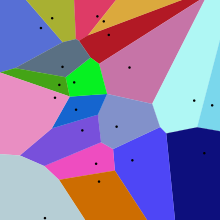
\includegraphics[scale=.7]{220px-Euclidean_Voronoi_diagram.svg.png}
  \caption{Celdas de Voronoi \cite{imgVOR}.} 
  \label{f5}
\end{figure}
\bigskip

\section{Objetivo}
De los códigos dados en el repositorio de Schaeffer \cite{dra} donde en el diagrama de Voronoi se generan las semillas aleatorias en un plano bidimensional y estas a su vez generan las celdas de distintos colores y aunado a esto una grieta o fisura que se propaga aleatoriamente su recorrido pero tiende a irse por las fronteras de las celdas, simulando así núcleos en algún proceso de cristalización en un material y la propagación de la grieta. A partir de esto se debe examinar de manera sistemática el efecto del número de semillas y del tamaño de la zona en la distribución en las grietas que se forman en términos de la mayor distancia manhattan entre la grieta y el exterior de la pieza \cite{elisa}.

\section{Simulación}
Para la práctica no se explicarán los códigos dados donde se crean las semillas, celdas y propagación de grieta ya que se pueden consultar en el repositorio de Schaeffer \cite{dra}. La simulación se enfoca en cómo se obtiene la distancia Manhattan desde el borde donde inicia la grieta hasta el punto más cercano al centro para saber qué tanto penetró la fractura a el material.
La programación completa se puede consultar en github \cite{Edson}. Lo primero que se realiza es el cambio automático del número de semillas en un ciclo \texttt{for} que tomará valores bajo, medio y alto, ya que en el programa dado se introduce un solo valor.

\begin{verbatim}
n, semillas = 40, []
for SEM in (5, 30, 100):
    k = SEM
    for s in range(k):
\end{verbatim}
A partir de este ciclo comienza el código donde se generan las semillas las celdas y la grieta, la lógica utilizada parte en que la grieta es color negro y el fondo son las celdas de colores entonces se construye la siguiente lógica en la cual se recorre la imagen cada píxel por fila y columna, condicionando que si en dicho píxel el color es igual a negro \texttt{(0, 0, 0)} entonces se guardará la coordenada de este, al final de la revisión de toda la imagen se obtiene la suma de píxeles color negro.
\begin{verbatim}
    for R in range(0,n):
            for S in range(0,n):
                columna1 = R
                fila1= S
                if g[columna1,fila1] == (0, 0, 0):
                    vectorX.append(R)
                    vectorY.append(S)
                    coordenada.append([R,S])
        total=(len(coordenada))# total de píxeles de grieta 
\end{verbatim}
Después de esto lo siguiente a realizar es todo el proceso en el que se determina el píxel que esta más lejos y el más cercano al centro de la imagen, para esto se realiza otro ciclo \texttt{for} en rango de la variable \texttt{total} que toma valor de la suma de las celdas encontradas en color negro, a cada coordenada de este se extrae el valor X y Y y el mismo procedimiento para la variable \texttt{origen} que se estableció como la mitad de la imagen en sus dos ejes. 
Esta separación es para poder utilizar cada dato en la determinación de la distancia Euclidiana ya que este método dió tanto distancia como coordenada del píxel mas cercano al centro sacando el mínimo de los acumulados en la variable \texttt{Eucl}. 

\begin{verbatim}
    for T in range(0, total):
        p=coordenada[T] 
        XS=p[0]         # obtengo X de la grieta 
        YS=p[1]         # obtengo Y de la grieta 
        origen = [((n-1)/2), ((n-1)/2)]
        OX = origen[0]
        OY = origen[1]
        DE= sqrt((XS-OX)**2+(YS-OY)**2) 
        Eucl.append((DE,coordenada[T])) 
        c=(min(Eucl))   # obtengo el píxel más cercano al centro 
        if XS== (n-1) or YS==(n-1):
            borde.append(coordenada[T])
        if XS==0 or YS==0:
            borde.append(coordenada[T])
    cercano=(c[1])      
    FX= cercano[0]
    FY= cercano[1]
    lejano=borde[0]
    IX=lejano[0]
    IY=lejano[1]
    DMx= fabs(FX-IX)
    DMy= fabs(FY-IY)
    DM = DMx + DMy       
    Manh.append(DM)
    
\end{verbatim}
Fuera del ciclo se utiliza la coordenada más cercana al centro y la más lejana al centro que es el inicio de la grieta por decir la que está en el borde, a estos se les extrae de igual manera en variables el valor de X y Y para sacar el valor absoluto entre X final menos X inicial y lo mismo para Y, para después sumar estos valores absolutos para tener la distancia Manhattan de el punto más lejano que llegó a penetrar en el material la propagación de la grieta. 

\section{Resultados}
Los resultados que se obtienen primeramente son las imágenes de la propagación de la grieta ahí se podrá observar de primera instancia si ésta pasó cerca del centro o tomó diferente camino, como se obtienen veinte imágenes de cada cantidad de semillas que son tres por matriz entonces se decidió hacer un gif realizados en la pagina giphy \cite{GIPHY} para cada situación y pueden ser encontrados en el repositorio de Samaniego en github \cite{Edson}.
También se obtuvieron datos como se puede observar en el cuadro \ref{tab1} donde se dividen las secciones en matrices y para cada una sus tres variantes de semillas, a cada sección se le hicieron veinte iteraciones para realizar el muestreo de el mínimo, máximo, promedio y media de la distancia (Manhattan) más lejana que se propago la grieta para ver si logró penetrar al centro de la matriz o imagen y ver el diferente comportamiento para número de semillas y dimensión de matriz. 

La última columna de datos observado en el cuadro \ref{tab1} llamada \texttt{Mayor al límite} refiere a las veinte iteraciones en las que hay una condición para que genere la grieta y esta condición es que si la grieta es muy pequeña menor al número de la zona (20, 40, 100, 200) entonces no va a interesar esa iteración y no generará la imagen, solo para las mayores a número de zona en la matriz, así esta columna registró que solo para la matriz 20x20 con un número alto de semillas (300) si cumplió con las veinte iteraciones.

    \begin{table}[H]
        \caption{Registro de mínimo, máximo, promedio y media de cada cantidad de semillas por matriz y cantidad de iteraciones realizadas superando el límite de cada matriz.}
        \bigskip
        \label{tab1}
        \centering
        \begin{tabular}{|r|r|r|r|r|r|r|}
        \hline
         Matriz& Semillas &Mín&Máx&Promedio&Media&Mayor al límite \\
        \hline
             & 5  & 0.0 & 18.0 & 8.5  & 9.0  & 16\\
        20x20& 80 & 2.0 & 17.0 & 10.9 & 12.5 & 15\\
             &300 & 3.0 & 22.0 & 12.9 & 13.5 & 20\\
        \hline
             & 5  & 5.0 & 36.0 & 18.3 & 17.0 & 18\\
        40x40& 30 & 1.0 & 38.0 & 17.7 & 20.0 & 17\\
             &100 & 2.0 & 36.0 & 18.7 & 20.0 & 16\\
        \hline
               & 30  & 3.0 & 63.0 & 21.5 & 17.0 & 10\\
        100x100&500  & 5.0 & 51.0 & 30.6 & 36.0 & 16\\
               &1500 & 3.0 & 61.0 & 21.2 & 17.5 & 8 \\ 
        \hline
               & 10 & 2.0 & 118.0 & 30.3 & 23.0 & 5 \\
        200x200&700 & 5.0 & 94.0  & 30.9 & 30.0 & 5 \\
               &3000& 3.0 & 72.0  & 29.9 & 23.5 & 9 \\
         \hline
        \end{tabular}
    \end{table}
Se logra determinar que conforme la zona o matriz crecía, las iteraciones que superaron el límite fue menor independientemente del número de semillas que se crearan debido a que se dió una cantidad alta de tres mil semillas para matriz de 200x200 eso quiere decir que debía propagarse más de 200 píxeles la grieta y no lo lograba.

Para una mejor representación de los mínimos, máximos y promedios de la grieta más cercana al centro se representa a continuación en diagramas caja bigote de cada matriz.
La figura \ref{f1} se observa que para poco número de semillas es menos probable que la grieta llegue al centro debido a que tiene menos fronteras por la cual se pueda desplazar la fractura, en cambio cuando aumentamos la cantidad de semillas a ochenta o trescientos se logra ver que el promedio de estos es muy similar debido a que hubo gran cantidad de iteraciones que se acercaron al centro pero solo en trescientas semillas fue que si hubo fractura al centro del material debido a que propago por más fronteras.

\begin{figure}[H]
  \centering      
  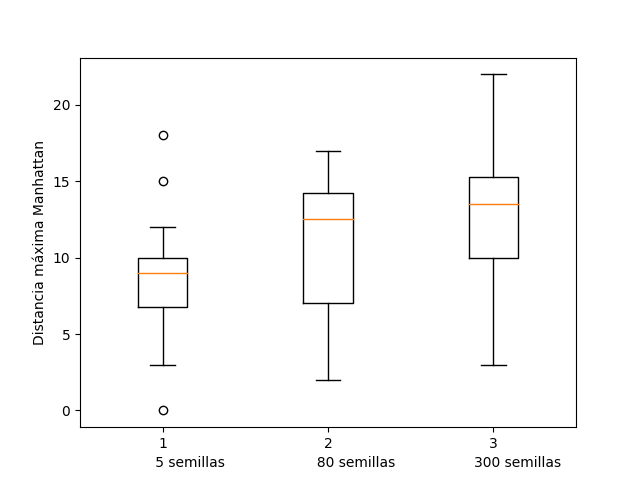
\includegraphics[scale=.7]{20x20.png}
  \caption{Diagrama caja-bigote de matriz 20x20.}
  \label{f1}
\end{figure}
\bigskip

\begin{figure}[H]
  \centering      
  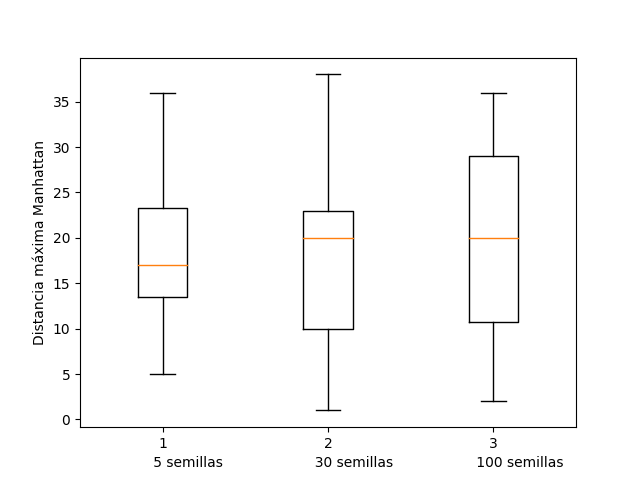
\includegraphics[scale=.7]{40x40.png}
  \caption{Diagrama caja-bigote de matriz 40x40.}
  \label{f2}
\end{figure}
\bigskip

\begin{figure}[H]
  \centering       
  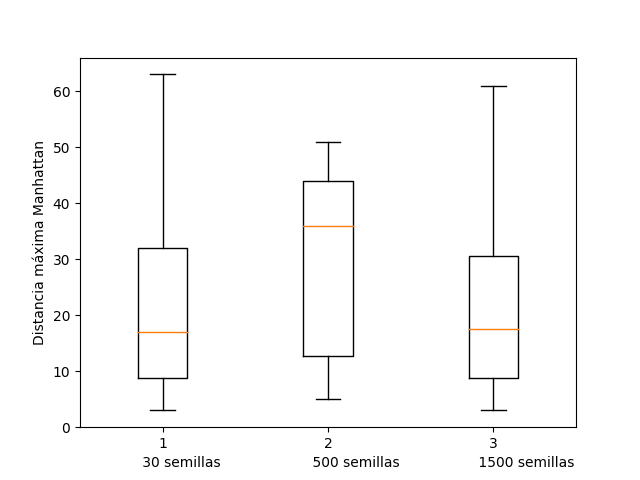
\includegraphics[scale=.7]{100x100.png}
  \caption{Diagrama caja-bigote de matriz 100x100.}
  \label{f3}
\end{figure}
\bigskip

\begin{figure}[H]
  \centering      
  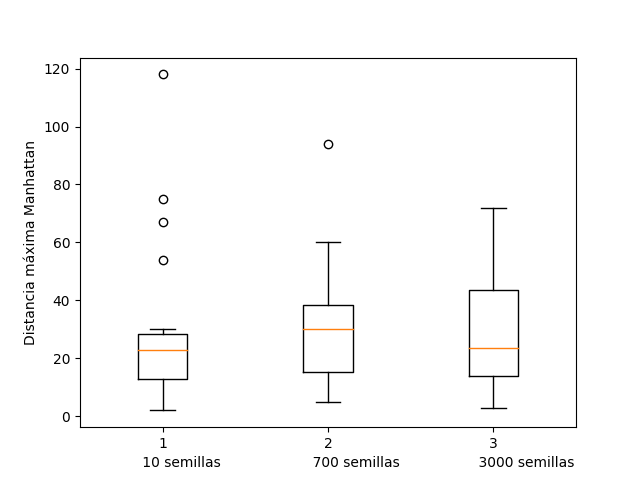
\includegraphics[scale=.7]{200x200.png}
  \caption{Diagrama caja-bigote de matriz 200x200.}
  \label{f4}
\end{figure}
\bigskip

En los diferentes casos de caja-bigote se llega a la conclusión de que a un número bajo de semillas si es más difícil la propagación de la grieta por lo que no fue muy común que esta llegara al centro aún que se aumentara la matriz como en la figura \ref{f4} donde con diez semillas solo una iteración se acercó mucho al centro pero las otras se mantuvieron lejanas y también es de detallar que para tres mil semillas no hubo mucho acercamiento al centro pero si hubo mayor aglomeración y repetibilidad en promedio.


\bibliography{refere}
\bibliographystyle{plainnat}




\end{document}
